\documentclass[mathserif,18pt,xcolor=table]{beamer}

% Load Beamer Style Theme
% TAMU Based
\usepackage{tamu_beamer}
% \usepackage[skip=0pt]{caption}

% \preto\subequations{\ifhmode\unskip\fi}
% \AtBeginEnvironment{subequations}{\ifhmode\unskip\fi}
% \AtBeginEnvironment{equation}{\ifhmode\unskip\fi}
\makeatletter
\g@addto@macro\normalsize{%
\setlength\abovedisplayskip{0pt}
\setlength\belowdisplayskip{0pt}
\setlength\abovedisplayshortskip{0pt}
\setlength\belowdisplayshortskip{0pt}
}
\makeatother


% Specifiy the location of images to be used
\graphicspath{{figures/}}

% ------------------------------------------------------------
% ------------------------------------------------------------
% ------------------------------------------------------------
% ----------------TITLE PAGE----------------------------------
% ------------------------------------------------------------
% ------------------------------------------------------------
% ------------------------------------------------------------
% Document Title Page
\title{Two-dimensional Plasmonic Devices}
% \subtitle{Preliminary Exam}
\author[Hasan Tahir Abbas]{Hasan Tahir Abbas\\~\\{\small {Supervised by: Dr. Robert D. Nevels}}}
\institute{Department of Electrical  \& Computer Engineering\\ \mbox{} \\ \pgfuseimage{tamuecenbig}}
\date[Spring 2017]{}
% ------------------------------------------------------------
% ------------------------------------------------------------
% ------------------------------------------------------------
% ------------------------------------------------------------
% ------------------------------------------------------------
% ------------------------------------------------------------
% ------------------------------------------------------------
% ------------------------------------------------------------
% ------------------------------------------------------------
% ------------------------------------------------------------
% ------------------------------------------------------------
% ------------------------------------------------------------
% ------------------------------------------------------------
% ------------------------------------------------------------
\begin{document}
\preto\subequations{\ifhmode\unskip\fi}
\AtBeginEnvironment{subequations}{\ifhmode\unskip\fi}
\AtBeginEnvironment{equation}{\ifhmode\unskip\fi}
% Draw Boxes in the footer with pertinent info
\tikzstyle{block} = [rectangle, draw, rounded corners, shade, top color=white, text width=5em,
bottom color=blue!50!black!20, draw=blue!40!black!60, very thick, text centered, minimum height=4em]
\tikzstyle{line} = [draw, -latex']
\tikzstyle{cloud} = [draw, ellipse,top color=white, bottom color=red!20, node distance=2cm, minimum height=2em]

% Tick Style
\beamertemplateballitem
% \beamertemplatetransparentcoveredhigh

\frame{\titlepage}


% Add TAMU logo on each slide in the north-east side
% Shifted to be right at the edge
%
% NOTE: Will have to compile twice
%
\addtobeamertemplate{frametitle}{}{%
\begin{tikzpicture}[remember picture,overlay]
  \node[anchor=north east,yshift=7pt,xshift=2pt] at (current page.north east) {
\includegraphics[height=.7cm]{ecen}};
\end{tikzpicture}}
% ------------------------------------------------------------
% ------------------------------------------------------------
% ------------------------------------------------------------
% ------------------------------------------------------------
% ------------------------------------------------------------
% ------------------------------------------------------------
% ------------------------------------------------------------
% ------------------------------------------------------------
% ------------------------------------------------------------
% ------------------------------------------------------------
% ------------------------------------------------------------
% ------------------------------------------------------------
% ------------------------------------------------------------
% ------------------------------------------------------------
\section{Outline}
\begin{frame}
  \frametitle{Outline}
  \framesubtitle{Preliminary Exam}
  \begin{itemize}
    \item Plasmonics Overview
    \item Background
    \item Theory and Methods
    \begin{itemize}
      \item[-]{Dispersion Relation}
      \item[-]{Computation of fields}
    \end{itemize}
    \item Results
    \item Proposed Work
  \end{itemize}
\end{frame}
% ------------------------------------------------------------
% ------------------------------------------------------------
% ------------------------------------------------------------
% ------------------------------------------------------------
% ------------------------------------------------------------
% ------------------------------------------------------------
% ------------------------------------------------------------
% ------------------------------------------------------------
% ------------------------------------------------------------
% ------------------------------------------------------------
% ------------------------------------------------------------
% ------------------------------------------------------------
% ------------------------------------------------------------
% ------------------------------------------------------------
\section{Overview}
% ------------------------------------------------------------
% ------------------------------------------------------------
\begin{frame}
  \frametitle{Plasmonics Overview}
  % ----------------------------------------------------------
  \begin{columns} % align columns
    \begin{column}{.5\textwidth}
      \begin{itemize}
        \item Utilizing the terahertz gap
        \item High electron mobility transistors (HEMTs)
        \item Two-dimensional materials
        \item Subwavelength Plasmonic waves
        \item Miniaturization of circuit and antenna devices
        \item Poor energy efficiencies
        \item Re-engineering of the transistor
      \end{itemize}
    \end{column}
    \begin{column}{.5\textwidth}
      % Use this to preserve fonts from Inkspace
      \begin{figure}
        \hspace*{-1cm}
        % \vspace*{-2cm}
        \def\svgwidth{1.2\linewidth}
        \input{figures/scale.pdf_tex}
        \caption{Typical GaAs/AlGaAs HEMT}
      \end{figure}
      \end{column}%
    \end{columns}
  \end{frame}
% ------------------------------------------------------------
% ------------------------------------------------------------
% ------------------------------------------------------------
% ------------------------------------------------------------
% ------------------------------------------------------------
% ------------------------------------------------------------
% ------------------------------------------------------------
% ------------------------------------------------------------
% ------------------------------------------------------------
% ------------------------------------------------------------
% ------------------------------------------------------------
% ------------------------------------------------------------
% ------------------------------------------------------------
% ------------------------------------------------------------
\section{Background}
% ------------------------------------------------------------
% ------------------------------------------------------------
% ------------------------------------------------------------
% ------------------------------------------------------------
% ------------------------------------------------------------
% ------------------------------------------------------------
% ------------------------------------------------------------
% ------------------------------------------------------------
% ------------------------------------------------------------
% ------------------------------------------------------------
% ------------------------------------------------------------
% ------------------------------------------------------------
% ------------------------------------------------------------
% ------------------------------------------------------------
\section{Background}
\begin{frame}
  \frametitle{Backrgound and Previous Work}
  \framesubtitle{Surface Plasmons}

  \begin{columns} % align columns
    \begin{column}{.5\textwidth}
      \begin{minipage}[T][.1\textheight][c]{\linewidth}
        \begin{itemize}
          \item Metal-dielectric interface
        \end{itemize}
          \begin{equation} \nonumber
            \mathrm{Re} \left[\E_{metal}\right](\O) < 0
          \end{equation}
          \begin{itemize}
            \item Slow surface waves
            \item Subwavelength Control of electromagnetic waves
            \item Focusing beyond the diffraction limit
          \end{itemize}
      \end{minipage}
      %
    \end{column}
    %
    \begin{column}{.5\textwidth}
      % Use this to preserve fonts from Inkspace
      \begin{figure}
        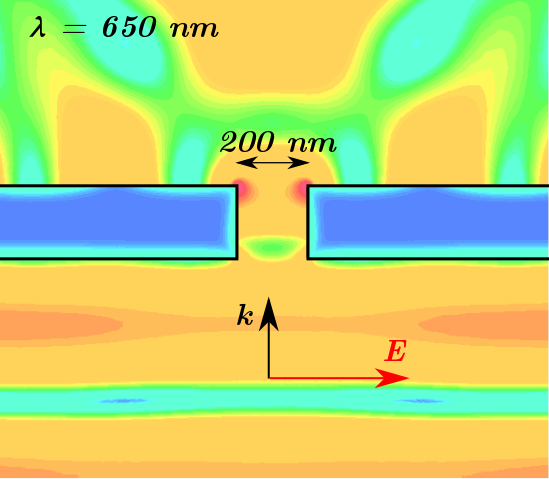
\includegraphics[scale=.3]{E_squared_final.png}
        \caption{Subwavelength Transmission through a Silver slit}
      \end{figure}
      \end{column}%
    \end{columns}
\end{frame}
% ------------------------------------------------------------
% ------------------------------------------------------------
% ------------------------------------------------------------
% ------------------------------------------------------------
% ------------------------------------------------------------
% ------------------------------------------------------------
% ------------------------------------------------------------
\begin{frame}
  \frametitle{Optical Nanoantennas}
  \framesubtitle{Dispersion Relation}
  \begin{columns}[T] % align columns
    \begin{column}{.5\textwidth}
      \begin{itemize}
        \item Metal-dielectric Interface
      \end{itemize}
      \begin{equation} \nonumber
        k_{sp}=\frac{\O}{c}\sqrt {\dfrac {\E_{1}\E_{2}(\O)} {\E_{1} + \E_{2}(\O)}}
        \label{eq:dis_spp}
      \end{equation}
      \begin{itemize}
        \item Accurate material description using Drude-critical points
      \end{itemize}
      \begin{equation} \nonumber
          \E_2(\O) = \E_{\inf} - \frac{\O_{d}^{2}}{\O^2 + j\gamma \O} + \sum \limits_{i = 1}^N G_i(\O)
        \label{eq:eps_drude_cp}
        \end{equation}
        \begin{equation} \nonumber
            G_i(\O) = C_i \left[ \frac{e^{j \phi_i}}{\O_i - \O - j \Gamma_i} + \frac{e^{-j \phi_i}}{\O_i + \O + j \Gamma_i} \right]
          \label{eq:CP_terms}
          \end{equation}
    \end{column}
    \begin{column}[T]{.5\textwidth}
      \begin{figure}
        \vspace*{-2cm}
        \includestandalone[width=.75\linewidth]{figures/ep_gold}
        \label{fig:ep_gold}
        \caption{Dispesion curve for Gold-air SPPs}
      \end{figure}
      \begin{figure}
        \vspace*{-1cm}
        \includestandalone[width=.75\linewidth]{figures/disp_gold}
        \label{fig:disp_gold}
      \end{figure}
    \end{column}
  \end{columns}
\end{frame}
% ------------------------------------------------------------
% ------------------------------------------------------------
% ------------------------------------------------------------
% ------------------------------------------------------------
% ------------------------------------------------------------
% ------------------------------------------------------------
% ------------------------------------------------------------
% ------------------------------------------------------------
\begin{frame}
  \frametitle{Backrgound and Previous Work}
  \framesubtitle{Optical Nanoantennas}

  \begin{columns} % align columns
    \begin{column}{.45\textwidth}
      % \begin{minipage}[T][.1\textheight][c]{\linewidth}
      \vspace*{-1cm}
      \begin{itemize}
        \item Convert Localized near-field to efficient far-field radiation
        \item Low Q-factor
        \item Extremely small size
        \item \color{red}{High Purcell Factor}
      \end{itemize}
      \begin{equation} \nonumber
        \mathrm{P}  = \frac{\mathrm{Q}}{\mathrm{V}}
      \end{equation}
      \begin{itemize}
        \item Directive radiation
      \end{itemize}
      % \end{minipage}
      %
    \end{column}
    %
    \begin{column}{.55\textwidth}
      \vspace*{-1cm}
      % Use this to preserve fonts from Inkspace
      \begin{figure}
        \hspace*{-1cm}
        \def\svgwidth{\linewidth}
        \input{figures/curto.pdf_tex}
        \caption{Optical resonant cavities for electric field enhancement}
      \end{figure}
      \end{column}%
    \end{columns}
  \end{frame}
% ------------------------------------------------------------
% ------------------------------------------------------------
% ------------------------------------------------------------
% ------------------------------------------------------------
% ------------------------------------------------------------
% ------------------------------------------------------------
% ------------------------------------------------------------
% ------------------------------------------------------------
\begin{frame}
  \frametitle{Backrgound and Previous Work}
  \framesubtitle{Optical Nanoantennas (contd.)}

  \begin{columns} % align columns
    \begin{column}{.45\textwidth}
      \begin{minipage}[T][.1\textheight][c]{\linewidth}
        \begin{itemize}
          \item Scaled-down microwave designs
          \begin{itemize}
            \item[-] Directivity: Yagi-Uda antenna
            \item[-] Broadband: Bowtie antenna
          \end{itemize}
        \end{itemize}
        \begin{figure}
          \includegraphics[scale=.03]{bowtie_field_map.png}
          % \caption{Subwavelength Transmission through a Silver slit}
        \end{figure}
      \end{minipage}
    \end{column}
    %
    \begin{column}{.55\textwidth}
      % Use this to preserve fonts from Inkspace
      \hspace*{-1cm}
      \vspace*{-1cm}
      \begin{figure}
        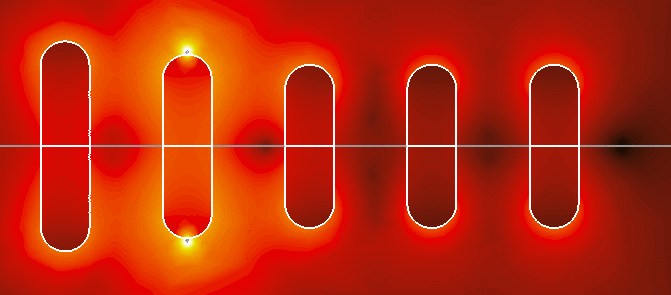
\includegraphics[scale=.04]{yagi_fields.png}
        % \caption{Subwavelength Transmission through a Silver slit}
      \end{figure}
      \hspace*{-1cm}
      \vspace*{-1.2cm}
      \begin{figure}

        \includegraphics[scale=.3]{yagi_patterna.png}
        % \caption{Subwavelength Transmission through a Silver slit}
      \end{figure}
      \end{column}%
    \end{columns}
\end{frame}
% ------------------------------------------------------------
% ------------------------------------------------------------
% ------------------------------------------------------------
% ------------------------------------------------------------
% ------------------------------------------------------------
% ------------------------------------------------------------
% ------------------------------------------------------------
% ------------------------------------------------------------
\begin{frame}
  \frametitle{Backrgound and Previous Work}
  \framesubtitle{Two-dimensional Electon Gas (2DEG)}

  \begin{columns} % align columns
    \begin{column}{.5\textwidth}
      \begin{minipage}[T][.1\textheight][c]{\linewidth}
        \begin{itemize}
          \item Semiconductor Heterostructure Interface
          \item High electron Mobility
          \item High concentration of electric charge
          \item \textbf{Two-dimensional Surface waves}
          \item Formation of Quantum Well
          \begin{itemize}
            \item[]{Two-dimensional confinement of electrons}
          \end{itemize}
        \end{itemize}
      \end{minipage}
      %
    \end{column}
    %
    \begin{column}{.5\textwidth}
      % Use this to preserve fonts from Inkspace
      \begin{figure}
        \def\svgwidth{\linewidth}
        \input{figures/hemt.pdf_tex}
        \caption{Typical GaAs/AlGaAs HEMT}
      \end{figure}
      \end{column}%
    \end{columns}
\end{frame}
% ------------------------------------------------------------
% ------------------------------------------------------------
% ------------------------------------------------------------
% ------------------------------------------------------------
% ------------------------------------------------------------
% ------------------------------------------------------------
% ------------------------------------------------------------
% ------------------------------------------------------------
\begin{frame}
  \frametitle{Backrgound and Previous Work}
  \framesubtitle{2DEG (contd.)}

  \begin{columns} % align columns
    \begin{column}{.5\textwidth}
      \begin{minipage}[T][.1\textheight][c]{\linewidth}
        \begin{itemize}
          \item Plasma waves in 2DEG
          \item Dyakonov-Shur instability
          \begin{itemize}
            \item[-]{Voltage bias at source and drain terminals}
            \item[-]{Plasma resonance}
            \item[-]{Emission of terahertz radiation}
            \item[-]{External radiation detection}
          \end{itemize}
          \item \emph{Electronic Flute}
          \item Tunable resonance with gate voltage
          \item Shallow water waves
          \begin{itemize}
            \item[-]{\color{red}Surface waves}
          \end{itemize}
        \end{itemize}
      \end{minipage}
      %
    \end{column}
    %
    \begin{column}{.5\textwidth}
      % Use this to preserve fonts from Inkspace
      \begin{figure}
        \def\svgwidth{\linewidth}
        \input{figures/flute_2deg.pdf_tex}
        % \caption{Typical GaAs/AlGaAs HEMT}
      \end{figure}
      \begin{equation} \nonumber
        \begin{split}
          \lambda &= \frac{c}{f} \\
                & \Longrightarrow  300 \u \mathrm{m}
        \end{split}
        \label{eq:disp_TE_two}
      \end{equation}
      \end{column}%
    \end{columns}
\end{frame}
% ------------------------------------------------------------
% ------------------------------------------------------------
% ------------------------------------------------------------
% ------------------------------------------------------------
% ------------------------------------------------------------
% ------------------------------------------------------------
% -------------------THEORY-----------------------------------
% ------------------------------------------------------------
% ------------------------------------------------------------
% ------------------------------------------------------------
% ------------------------------------------------------------
% ------------------------------------------------------------
% ------------------------------------------------------------
% ------------------------------------------------------------
% ------------------------------------------------------------
% ------------------------------------------------------------
% Beginning of the actual content
\section{Theory}
\begin{frame}
  \frametitle{Theory}
  \framesubtitle{2DEG formation}
  \begin{columns} % align columns
    \begin{column}{.5\textwidth}
      \begin{minipage}[T][.1\textheight][c]{\linewidth}
        \begin{itemize}
          \item Semiconductor Heterostructure Interface
          \item High electron concentration
          \item \textbf{Two-dimensional Surface waves}
          \item Formation of Quantum Well
          \begin{itemize}
            \item[]{Two-dimensional confinement of electrons}
          \end{itemize}
        \end{itemize}
      \end{minipage}
      %
    \end{column}
    %
    \begin{column}{.5\textwidth}
      % Use this to preserve fonts from Inkspace
      \begin{figure}
        \vspace*{-1cm}
        \def\svgwidth{\linewidth}
        \input{figures/2deg_bandgap.pdf_tex}
        \caption{Band diagram of a GaAs/AlGaAs heterostructure}
      \end{figure}
      \begin{itemize}
        \item[]{\makebox[.5cm][l]{$E_c$} - Conduction band edge}
        \item[]{\makebox[.5cm][l]{$E_f$} - Fermi level}
      \end{itemize}
      \end{column}%
    \end{columns}
  \end{frame}
  % ------------------------------------------------------------
  % ------------------------------------------------------------
  % ------------------------------------------------------------
  % ------------------------------------------------------------
  % ------------------------------------------------------------
  % ------------------------------------------------------------
  % ------------------------------------------------------------
  \begin{frame}

    \frametitle{Theory}
    \framesubtitle{2DEG Dispersion Relation}
    \vspace*{-.5cm}
    \begin{columns} % align columns
      \begin{column}[T]{.5\textwidth}
        \begin{itemize}
          \item TE mode
        \end{itemize}
        \begin{equation} \nonumber
          k_{z1} + k_{z2} = \O \sigma_s(\O)
          \label{eq:disp_TE_two}
        \end{equation}
        \begin{itemize}
          \item[] No real solutions for an isotropic environment
        \end{itemize}
        \begin{itemize}
          \item TM mode
        \end{itemize}
        \begin{equation} \nonumber
          \tcbhighmath[drop fuzzy shadow]{\frac{\E_1(\O)}{k_{z1}} + \frac{\E_2(\O)}{k_{z2}} = -\frac{\sigma_s(\O)}{\O}}
          \label{eq:disp_TM_two}
        \end{equation}
        \begin{itemize}
          \item[] Real solution(s). Surface waves exist.
        \end{itemize}
      \end{column}
      %
      \begin{column}[T]{.5\textwidth}
        \begin{equation} \nonumber
          \begin{split}
            k_{zi} = \sqrt{\left(\frac{\O}{c}\right)^2 \E_i(\O) -  k_x^2}
          \end{split}
          \label{eq:kz}
        \end{equation}
        % Use this to preserve fonts from Inkspace
        \begin{figure}
          \def\svgwidth{\linewidth}
          \input{figures/2deg.pdf_tex}
          \caption{2DEG at a semiconductor heterojunction}
        \end{figure}
        \end{column}%
      \end{columns}
    \end{frame}
    % ------------------------------------------------------------
    % ------------------------------------------------------------
    % ------------------------------------------------------------
    % ------------------------------------------------------------
    % ------------------------------------------------------------
    % ------------------------------------------------------------
    % ------------------------------------------------------------
    \begin{frame}
      \frametitle{Theory}
      \framesubtitle{Material Description}
      \begin{columns}[T] % align columns
        \begin{column}{.5\textwidth}
          \begin{itemize}
            \item Complex valued
            \item Drude-Lorentz oscillator model
          \end{itemize}
          \begin{equation} \nonumber
            \E(\O) = \E^{\inf} + \prod_i\frac{\O_{li}^2 - \O^2 - j\gamma_{li} \O}{\O_{ti}^2 - \O^2 - j\gamma_{ti} \O}
            \label{eq:eps}
          \end{equation}
          \begin{itemize}
            \item[]{\makebox[.3cm][l]{$\E^{\inf}$} - High-frequency limit}
            \item[]{\makebox[.3cm][l]{$\O_{ti}$} - TO phonon frequencies}
            \item[]{\makebox[.3cm][l]{$\O_{li}$} - LO phonon frequencies}
            \item[]{\makebox[.3cm][l]{$\gamma$} - Damping constants}
          \end{itemize}
        \end{column}
        \begin{column}[T]{.5\textwidth}
          \begin{figure}
            \vspace*{-2cm}
            \subfloat[]{\includestandalone[width=.65\linewidth,keepaspectratio]{figures/epsilon_gaas}
            \label{fig:eps_Ga}}
            \vspace*{0cm}
            \subfloat[Dispersion curve]{\includestandalone[width=.65\linewidth,keepaspectratio]{figures/dispersion_gaas}
            \label{fig:eps_Sto}}
            % \caption{Dielectric Functions of the materials in bulk form. Solid line: real part, dashed line: imaginary part}
            % \label{fig:eps}
          \end{figure}
          \end{column}%
        \end{columns}
      \end{frame}
      % ------------------------------------------------------------
      % ------------------------------------------------------------
      % ------------------------------------------------------------
      % ------------------------------------------------------------
      % ------------------------------------------------------------
      % ------------------------------------------------------------
      % ------------------------------------------------------------
      \begin{frame}
        \frametitle{Theory}
        \framesubtitle{Thin Sheet Simulation}
        \begin{columns}[T] % align columns
          \begin{column}{.5\textwidth}
            \begin{itemize}
              \item{Impedance (Leontovich) Boundary Conditions}
              \end{itemize}
              \begin{equation} \nonumber
                \v E_{tan} = \eta Z_0 \hat{\v n} \times \v H
                \label{eq:eps}
              \end{equation}
              \begin{itemize}
                \item[]{\makebox[.3cm][l]{$\eta$} - Normalized impedance ($Z/Z_0$)}
                \item[]{\makebox[.3cm][l]{$Z_0$} - free space impedance}
              \end{itemize}
              \begin{itemize}
              \item{Volume Integral formulation}
              \item{Internal fields described by volume current denstity $J_v$}
              \item{Surface current $J_s$ approximated from $J_v$}
            \end{itemize}
          \end{column}
            \begin{column}[T]{.5\textwidth}
              \begin{itemize}
                \item{Impedance (Leontovich) Boundary Conditions}
                \end{itemize}
                \begin{equation} \nonumber
                  \v E_{tan} = \eta Z_0 \hat{\v n} \times \v H
                  \label{eq:eps}
                \end{equation}
              % Use this to preserve fonts from Inkspace
              \begin{figure}
                \def\svgwidth{\linewidth}
                \input{figures/seniors.pdf_tex}
                \caption{Dielectric Slab geometry}
              \end{figure}
            \end{column}%
          \end{columns}
        \end{frame}
        % ------------------------------------------------------------
        % ------------------------------------------------------------
        % ------------------------------------------------------------
        % ------------------------------------------------------------
        % ------------------------------------------------------------
        % ------------------------------------------------------------
        % ------------------------------------------------------------
        \begin{frame}
          \frametitle{Theory}
          \framesubtitle{Thin Sheet proposed solution}
          \begin{columns}[T] % align columns
            \begin{column}{.5\textwidth}
              \begin{itemize}
                \item{Surface Equivalence Theorem}
                \end{itemize}
                \begin{equation} \nonumber
                  \v E_{tan} = \eta Z_0 \hat{\v n} \times \v H
                  \label{eq:eps}
                \end{equation}
                \begin{itemize}
                  \item[]{\makebox[.3cm][l]{$\eta$} - Normalized impedance ($Z/Z_0$)}
                  \item[]{\makebox[.3cm][l]{$Z_0$} - free space impedance}
                \end{itemize}
                \begin{itemize}
                \item{Internal fields described by volume current denstity $J_v$}
                \item{Surface current $J_s$ approximated from $J_v$}
              \end{itemize}
            \end{column}
              \begin{column}[T]{.5\textwidth}
                % Use this to preserve fonts from Inkspace
                \begin{figure}
                  \def\svgwidth{\linewidth}
                  \input{figures/seniors.pdf_tex}
                  \caption{Dielectric Slab geometry}
                \end{figure}
              \end{column}%
            \end{columns}
          \end{frame}
      % ------------------------------------------------------------
      % ------------------------------------------------------------
      % ------------------------------------------------------------
      % ------------------------------------------------------------
      % ------------------------------------------------------------
      % ------------------------------------------------------------
      % ------------------------------------------------------------

      \begin{frame}
        \frametitle{Results}
        \framesubtitle{Thin Sheet Simulation ($TM_z$)}
        \begin{columns}[T] % align columns
          \begin{column}{.5\textwidth}
            \begin{itemize}
              \item[-]{$TM_z$ polarization}
              \item[-]{Dielectric Rod of length 2.5 $\lambda$}
              \item[-]{$\E = 4$, $\u = 1$}
            \end{itemize}
            \begin{figure}[h]
              \normalsize
              \centering
              \includestandalone[width=\textwidth]{figures/tm_plate}
              \caption{Thin sheet under $\mathrm{TM_z}$ polarized plane wave incidence}
              \label{fig:tm_plate}
            \end{figure}
          \end{column}
          \begin{column}[T]{.5\textwidth}
            \begin{figure}
              \vspace*{-2cm}
              \includestandalone[width=\linewidth,keepaspectratio]{figures/richmond_tm2}
              \caption{Radar Cross-section}
              \label{fig:TM_rcs}
            \end{figure}
            \end{column}%
          \end{columns}
        \end{frame}
        % ------------------------------------------------------------
        % ------------------------------------------------------------
        % ------------------------------------------------------------
        % ------------------------------------------------------------
        % ------------------------------------------------------------
        % ------------------------------------------------------------
        % ------------------------------------------------------------
        \begin{frame}
          \frametitle{Results}
          \framesubtitle{Thin Sheet Simulation ($TE_z$)}
          \begin{columns}[T] % align columns
            \begin{column}{.5\textwidth}
              \begin{itemize}
                \item[-]{$TE_z$ polarization}
                \item[-]{Dielectric Rod of length 2.5 $\lambda$}
                \item[-]{$\E = 4$, $\u = 1$}
              \end{itemize}
              \begin{figure}[h]
                \normalsize
                \centering
                \includestandalone[width=\textwidth]{figures/te_plate}
                \caption{Thin sheet under $\mathrm{TE_z}$ polarized plane wave incidence}
                \label{fig:te_plate}
              \end{figure}
            \end{column}
            \begin{column}[T]{.5\textwidth}
              \begin{figure}
                \vspace*{-2cm}
                \includestandalone[width=\linewidth,keepaspectratio]{figures/richmond_te1}
                \caption{Radar Cross-section}
                \label{fig:TE_rcs}
              \end{figure}
              \end{column}%
            \end{columns}
          \end{frame}

\end{document}
